\chapter{Reservoir Computing}\label{ch:reservoir-computing}

At a high level, an RC is a method to transform one time-varying
signal $\bm{u}(t)$, the input to the RC, into another time-varying
signal $\bm{y}(t)$, the output of the RC. The RC is constructed in
such a way that, given an example input and a desired output, the RC
can be \emph{trained} to produce that output when given the
corresponding input. Once trained, the RC can then be used to perform
the trained transformation on inputs it has not seen before.

The RC does this by means of an internal dynamic system called the
\emph{reservoir}, which is coupled to the input $\bm{u}(t)$. If the
reservoir's dynamics can be expressed as a first-order differential
equation, which covers a broad range of interesting choices of
reservoir, then the reservoir's internal state $\bm{r}$ is given by
\begin{equation}
  \label{eq:reservoir}
  \dot{\mathbf{r}}(t) = \mathbf{R}\left(\mathbf{r}, \mathbf{u}, t\right),
\end{equation}
where $\mathbf{R}$ defines the dynamics of the reservoir.

Thie reservoir is commonly a specific type of system called an
\emph{echo state network}, discussed in \cref{sec:esn}, but this is
not at all a requirement. Effective RCs have been built around
autonomous Boolean networks~\cite{canaday2018}, optical feedback
systems~\cite{antonik2016}, single time-delay Boolean
nodes~\cite{haynes2015}, and many others. The specific properties that
a reservoir must have in order to produce a functioning RC is an open
question. Though there are a few known results, which I will discuss
in \cref{sec:reservoir-properties}, the most direct and practical way
to know if a given reservoir will work is to build, train, and test
it.

The output $\bm{y}(t)$ of the RC is constructed from a linear
combination of a set of \emph{read-out} signals constructed from the
reservoir state $\bm{r}(t)$ by means of a read-out function $\bm{g}$,
\begin{equation}
  \label{eq:output}
  \bm{y}(t) = W_\text{out}\;\bm{g}\left(\bm{r}(t)\right).
\end{equation}
This is called the RCs \emph{output layer}. Often, $\bm{g}$ is the
identity function, and the output signal $\bm{y}(t)$ is a direct
linear combination of the state variables of the reservoir. However, a
non-identity $\bm{g}$ can be used to break an unwanted symmetry in the
$\bm{u}$-to-$\bm{y}$ transformation, or to model incomplete
measurements of a physical system being used as a reservoir.

% FIXME figure for generic reservoir

Together, \cref{eq:reservoir} and \cref{eq:output} define a reservoir
computer, and define the transformation from input signal $\bm{u}(t)$
to output $\bm{y}(t)$.

Intuitively, the input signal $\bm{u}(t)$ drives the reservoir,
producing a large number of reservoir state signals $\bm{r}(t)$. These
state signals may be quite complicated, and likely none of them match
the desired transformation, but they are combined by means of
$W_\text{out}$ to produce the desired transformation. The reservoir's
purpose is to broadcast the input signal into a high-dimensional
space, and the output layer's purpose is to combine those many dimensions
into the meaningful desired output of the RC.

The reservoir dynamics $\bm{R}$ and the readout function $\bm{g}$ are
considered a fixed part of the RCs construction, and are not part of
the training process. I will discuss this choice in more detail in
\cref{sec:esn,sec:reservoir-properties}. Once these design parameters
are fixed, the weight matrix $W_\text{out}$ can be calculated from an
example input and an example output by a process called
\emph{training}, which results in an RC that performs the desired
transformation.

\section{Training an RC}\label{sec:training}

Training an RC starts with an example input signal
$\bm{u}_\text{train}(t)$ and corresponding example output signal
$\bm{y}_\text{train}(t)$. As an example, $\bm{u}_\text{train}(t)$ might be
the $x$ and $y$ components of a three-dimensional dynamic system, and
$\bm{y}_\text{train}(t)$ would be the $z$ component. An RC trained on this
example would learn how to infer the $z$ component of the system from
the other two.

The first step is to feed the example input $\bm{u}_\text{train}(t)$ into the reservoir, producing an example reservoir response $\bm{r}_\text{train}(t)$. Using \cref{eq:output}, the final goal of training is to find a $W_\text{out}$ such that
\begin{equation}
  \label{eq:approx-output}
  \mathbf{y}_\text{train}(t) \approx W_\text{out}\;\mathbf{g}\left(\mathbf{r}_\text{train}(t)\right).
\end{equation}

For many practical reservoirs, it takes some time for the reservoir
state $\bm{r}(t)$ to synchronize with the input $\bm{u}(t)$. During
this time, the reservoir state still depends on its initial condition,
and so is unsuitable for use as training data. Practically, if the
example data starts at $t = 0$, then all the data before $t <
t_\text{warmup}$ is discarded, and the approximation in
\cref{eq:approx-output} need only be true for $t >
t_\text{warmup}$. The warmup time $t_\text{warmup}$ will depend on the
specific choice of reservoir in the RC.

The right-hand side of \cref{eq:approx-output} is linear in
$W_\text{out}$, and can be solved by any number of linear regression
methods. For RCs, $W_\text{out}$ is most commonly found via ridge
regression, also known as Tikhonov regularization, which chooses
$W_\text{out}$ to minimize
\begin{equation}
  \label{eq:ridge}
  \sum_{t>t_\text{warmup}} |\mathbf{u}_\text{train}(t) - W_\text{out}\;\mathbf{r}_\text{train}(t)|^2 + \alpha ||W_\text{out}||^2.
\end{equation}
In most practical applications, the signals involved are either
measured at a fixed time step, or integrated at a fixed time step, and
the sum in \cref{eq:ridge} is understood to be over these fixed time
steps.

The ridge parameter $\alpha$ is included to prevent overfitting, and
to help the RC generalize from the example input to unknown inputs. In
practice, this value depends on the scale of the input signal
$\bm{u}_\text{train}(t)$; for roughly unit-scale inputs, $\alpha$ may be
anywhere from $10^-{9}$ to $10^9$. Since the ridge regression can be
calculated quickly, and the result is only logarithmically sensitive
to the value of $\alpha$, the best value for $\alpha$ can be found
simply by grid search or cross-validation on the example input.

% FIXME better cite
The fact that training an RC amounts to a linear regression is a major
feature worth highlighting. Linear regressions are very fast, compared
to other machine learning techniques like gradient descent and
backpropogation~\cite{lukosevicius2009}. As a result, training an RC
is also fast. This opens the door to many interesting applications
where the ability to retrain the RC to a new system without the aid of
a supercomputer is desirable. For example, an RC that controls the
motors on an airborn drone could retrain itself in the event of a
mechanical failure.

\section{Forecasting with an RC}\label{sec:forecasting}

One of the primary uses of an RC is \emph{system forecasting}, where
the RC is primed with an input signal from a dynamic system and then
switched into a free-running mode, where it produces a future forecast
of that signal. This is most commonly used to to forecasting for
chaotic systems, where forecasting is definitionally difficult.

Training an RC for forecasting starts with an example input signal
$\bm{u}_\text{train}(t)$, but does not need an example output
$\bm{y}_\text{train}(t)$ as in normal training. As before, feeding the
example input into the reservoir generates an example reservoir
response $\bm{r}_\text{train}(t)$. For forecasting, however, the matrix
$W_\text{out}$ is chosen so that
\begin{equation}
  \label{eq:approx-output-forecast}
  \mathbf{u}_\text{train}(t) \approx W_\text{out}\;\mathbf{g}\left(\mathbf{r}_\text{train}(t)\right).
\end{equation}
That is, the RC is trained to reproduce its input as its output,
\begin{equation}
  \label{eq:approx-output-input}
  \bm{u}(t) \approx \bm{y}(t).
\end{equation}
As before, this $W_\text{out}$ is found via ridge regression.

Once trained in this way, the RC can be used for forecasting. First,
the RC is primed with an input signal $\bm{u}(t)$ to be used as the
basis for forecasting. This priming step synchorizes the reservoir
state $\bm{r}(t)$ to the input, and intuitively provides the RC with
the past history it will draw on to produce the forecast. This is a
warmup step, similar to that used during training. At the moment
forecasting begins, the approximation \cref{eq:approx-output-input} is
substituted in to the reservoir equation \cref{eq:reservoir},
effectively connecting the input of the RC to the output. The RC now
evolves forward in time according to
\begin{equation}
  \label{eq:reservoir-auto}
  \dot{\mathbf{r}}(t) = \mathbf{R}\left(\mathbf{r}, W_\text{out}\;\bm{g}(\bm{r}), t\right),
\end{equation}
Note that this RC no longer has any external input and runs
autonomously. The RC output $\bm{y}(t)$, calculated as usual from the
output layer in \cref{eq:output}, is the forecasted signal.

\section{Echo State Networks}\label{sec:esn}

% FIXME cite echo state more
Although there are many choices for the dynamic reservoir at the heart
of an RC, the reservoir computing method originated as a practical way
to train recurrent neural networks~\cite{lukosevicius2009}, by only
training the weights in the output layer. One such network reservoir
design, known as an echo state network (ESN)~\cite{jaeger2001},
remains popular and will be my choice of dynamic reservoir for this
thesis.

An echo state network is composed of number of nodes $N$. Each node in
the network has a number of inputs, drawn either from other nodes in
the network or from the external driving system. Each node also has an
internal state, a single value that decays exponentially to zero over
time with a decay rate $\gamma$. The node's inputs are summed together
with weights, and this sum is passed through an activation function
$f$ to produce a driving signal to the node's exponential state, which
is used as the node's output.

The input connections and weights for each node are represented by two
matrices: $W_\text{in}$, for connections from the overall input
$\bm{u}(t)$, and $W_r$, for recurrent connections to other nodes
inside the network. For example, $W_{r,i,j}$ represents a connection
from node $j$ inside the network to node $i$, while
$W_{\text{in},i,j}$ represents a connection from input component
$u_j(t)$ to node $i$. This means that $W_r$ is a $N \times N$ matrix,
while $W_\text{in}$ is an $N \times d$, where $d$ is the dimension of
the input signal $\bm{u}(t)$.

\begin{figure}
  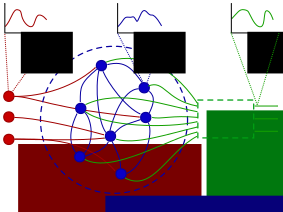
\includegraphics[width=0.6\textwidth]{figures/reservoir}
  \caption{High-level view of an echo state network RC. Each node may
    have two kinds of input connections: connections to other nodes in
    the network ($W_r$, blue), connections to the overall input
    ($W_\text{in}$, red). Each node may also have output connections
    to the overall output ($W_\text{out}$, green). Note that the
    internal connections may contain cycles.  When the RC is used to
    perform forecasting, the output on the right side is connected to
    the input on the left side, allowing the RC to run autonomously
    with no external input.}%
  \label{fig:reservoir}
\end{figure}

Put together, the dynamics of an echo state network RC are
\begin{align}
  \label{eq:esn}
  \dot{\bm{r}}(t) &= - \gamma \bm{r}(t) + \gamma \bm{f}\left( W_r\;\bm{r}(t) + W_\text{in}\;\bm{u}(t) \right), \\
  \bm{y}(t) &= W_\text{out}\;\bm{g}\left(\bm{r}(t)\right), \nonumber
\end{align}
where the vector function $\bm{f}$ is understood to mean applying the
one-dimensional activation function $f$ component-by-component. This
construction is summarized in \cref{fig:reservoir}. I will discuss
choosing the matrices $W_\text{in}$ and $W_r$, the parameter $\gamma$,
and the activation function $f$ in \cref{sec:esn-construction}.

This is the continuous-time formulation of an ESN. It is also common
to see a discrete-time formulation, which can be derived simply from
\cref{eq:esn} by the application of forward Euler
integration. Additionally, the forecasting method described in
\cref{sec:forecasting} involves a modification to the RC equation once
the RC is trained. These variations on the ESN equation are summarized
in \cref{tab:esn}.

\begin{table}
  \caption{A summary of variations of the ESN equation. The
    discrete-time formulation is the result of Euler-integrating the
    continuous-time formulation, and the forecasting variant is
    derived via the substitution described in \cref{sec:forecasting}.}
  \begin{tabular}{lrl}
    Variation Name & & Equations \\
    \hline
    \rule{0pt}{4ex}
    Continuous Time & $\bm{\dot{r}}(t) =$ & $- \gamma \bm{r}(t) + \gamma \bm{f}\left( W_r\;\bm{r}(t) + W_\text{in}\;\bm{u}(t) \right)$ \\
    (inference) & $\bm{y}(t) =$ & $W_\text{out}\;\bm{g}\left(\bm{r}(t)\right)$ \\
    \rule{0pt}{4ex}
    Continuous Time & $\bm{\dot{r}}(t) =$ & $- \gamma \bm{r}(t) + \gamma \bm{f}\left( W_r\;\bm{r}(t) + W_\text{in}\;W_\text{out}\;\bm{g}\left(\bm{r}(t)\right) \right)$ \\
    (forecasting) & $\bm{y}(t) =$ & $W_\text{out}\;\bm{g}\left(\bm{r}(t)\right)$ \\
    \rule{0pt}{4ex}
    Discrete Time & $\bm{r}(t + \Delta t) =$ & $(1 - \gamma \Delta t) \bm{r}(t) + \gamma \Delta t \bm{f}\left( W_r\;\bm{r}(t) + W_\text{in}\;\bm{u}(t) \right)$ \\
    (inference) & $\bm{y}(t) =$ & $W_\text{out}\;\bm{g}\left(\bm{r}(t)\right)$ \\
    \rule{0pt}{4ex}
    Discrete Time & $\bm{r}(t + \Delta t) =$ & $(1 - \gamma \Delta t) \bm{r}(t) + \gamma \Delta t \bm{f}\left( W_r\;\bm{r}(t) + W_\text{in}\;W_\text{out}\;\bm{g}\left(\bm{r}(t)\right) \right)$ \\
    (forecasting) & $\bm{y}(t) =$ & $W_\text{out}\;\bm{g}\left(\bm{r}(t)\right)$ \\
  \end{tabular}
  \label{tab:esn}
\end{table}

% FIXME cite \gamma \Delta t = 1
The Euler integration is only an accurate representation of
\cref{eq:esn} when $\gamma \Delta t \ll 1$. However, many authors will
take $\gamma \Delta t = 1$. Although this is no longer an accurate
approximation to the continuous-time ESN in \cref{eq:esn}, these
discrete-time ESNs still function well as an RC. That the RC is not
sensitive to this kind of fundamental change in the underlying
reservoir is a hallmark of the RC method. The specific form of the
underlying reservoir is largely unimportant, except for a few
requirements to be discussed in
\cref{sec:reservoir-properties}. Indeed, the internal structure of an
ESN is determined randomly!

\section{Constructing ESNs}\label{sec:esn-construction}

The parameters $W_r$, $W_\text{in}$, $\gamma$, and $f$ in
\cref{eq:esn} must be set before the ESN construction is complete. Of
these, $\gamma$ has the most simple interpretation: it controls the
exponential decay of the value of each node in the network. If this
rate is too slow, the reservoir will not be able to react fast enough
to its input to be useful for computing the output; if this rate is
too fast, the reservoir will respond immediately to its inputs and
have no useful memory of past inputs, which may be necessary for the
RC's task. As the reservoir network may contain cycles, there is also
the possibility that a high decay rate may result in very rapid
oscillation in the network, which is undesirable if the RC's desired
output does not contain such oscillation. In practice, this decay rate
should be matched to the characteristic timescale of the output
signal, and then can be manually tuned from there if needed.

If the read-out function $\bm{g}$ is taken to be the identity
function, as is common, and the activation function $f$ is linear,
then the forecasting-mode equations in \cref{tab:esn} are completely
linear and have simple, oscillatory analytic solutions. These are
known as \emph{linear RCs}. Linear RCs are mathematically easy to work
with, and as a result many of the known proofs about RCs are in the
context of linear RCs. One of the most recent and prominent results is
discussed further in \cref{ch:nvar}.

However, because the solutions to a linear RC in prediction mode are
so simple, it is not possible for them to reproduce the strange
attractors of chaotic systems. To do this, the activation function $f$
is used to introduce non-linearity into the equations. The most common
choice is the hyperbolic tangent, $f(x) = \tanh(x)$, and this will be
used in this thesis. This satisfies the non-linearity requirement, and
also ensures that each component of $\bm{r}(t)$ is bounded in $(-1,
1)$. Bounds on $\bm{r}(t)$ ensure that \cref{eq:esn} is particularly
well-behaved for numerical integrators. These bounds can also be used
to put bounds on the output $\bm{y}(t)$, which may be useful if that
output is driving a real-world system.

It is also possible to leave $f$ linear, and introduce non-linearity
into the system with $\bm{g}$. These \emph{output-layer nonlinear RCs} are
also discussed further in \cref{ch:nvar,ch:nvar-application}.

The matrices $W_r$ and $W_\text{in}$, and therefore the topology and
weights of the ESN, are chosen randomly. There are many random schemes
in use, from Erd{\"{o}}s-R{\'{e}}nyi networks and small-world
networks\cite{haluszczynski2019} to simpler cycle and line
networks.\cite{rodan2011} The scheme I use is simple. Although this
thesis only discusses RCs simulated in software, this scheme was
designed with an eye towards hardware implementation, where the number
of inputs to each node, and the total number of connections in the
network, have an associated hardware cost.

For the internal connections $W_r$, I generate a random network where
every node has a fixed number of inputs, or \emph{in-degree}, $k$. For
each node, I select $k$ nodes in the network without replacement and
use those as inputs to the current node. Each input is assigned a
random weight drawn from a normal distribution with mean $0$ and
variance $1$. This results in a connection matrix $W_r'$ where each
row has exactly $k$ non-zero entries. Finally, I rescale the whole
matrix
\begin{equation}
  \label{eq:setradius}
  W_r = \frac{\rho_r}{\operatorname{SR}(W_r')}\;W_r',
\end{equation}
where $\operatorname{SR}(W_r')$ is the spectral radius, or maximum
absolute eigenvalue, of the matrix $W_r'$. This scaling ensures that
$\operatorname{SR}(W_r') = \rho_r$, and $\rho_r$ is used to tune the
overall scale of the recurrent weights, and therefore the importance
of recurrent connections inside the network.

For $W_\text{in}$, I randomly connect each node to each RC input in
$\bm{u}(t)$ with probability $\sigma$. The weight for each connection
is drawn randomly from a normal distribution with mean $0$ and
variance $\rho_\text{in}^2$.

Together, $\sigma$ and $\rho_\text{in}$ are enough to generate a
random instantiation of $W_\text{in}$, and $k$ and $\rho_r$ are enough
to generate a random instantiation of $W_r$. The relative scales
$\rho_r$ and $\rho_\text{in}$ determine the importance of the
recurrent and external inputs, respectively. The entire construction
is reduced to choosing these \emph{metaparameters}, summarized in
\cref{tab:esn-metaparameters}.

\begin{table}
  \caption{Summary of echo state network metaparameters. These
    parameters must be chosen to produce a random realization of an
    ESN-based RC.}
  \begin{tabularx}{\linewidth}{rlX}
    & Parameter & Description \\
    \hline
    \rule{0pt}{4ex}
    $\gamma$ & Leak Rate & controls the exponential decay of each node. \\
    \rule{0pt}{4ex}
    $\sigma$ & Input Connectivity & the probability that any given input is connected to any given node. \\
    \rule{0pt}{4ex}
    $\rho_\text{in}$ & Input Scale & the variance of the normally-distributed input connection weights. \\
    \rule{0pt}{4ex}
    $k$ & Recurrent Connectivity & the number of input connections each node draws from other nodes in the network. \\
    \rule{0pt}{4ex}
    $\rho_r$ & Recurrent Scale & the spectral radius of $W_r$. This controls the scale of recurrent connection weights. \\
    \rule{0pt}{4ex}
    $f$ & Activation Function & the function computed at each node. This is usually $\tanh$. \\
    \rule{0pt}{4ex}
    $\bm{g}$ & Read-out Function & the output layer read-out. This is usually the identity function. \\
  \end{tabularx}
  \label{tab:esn-metaparameters}
\end{table}

\section{Properties of Good Reservoirs}\label{sec:reservoir-properties}

Which dynamic systems make for good reservoirs, and what properties
are desired in a reservoir, remains an open question. There are a
handful of known desirable properties that are used to guide reservoir
design, and in particular ESN design. Chief among these is the
\emph{fading memory property}, which states that the reservoir's
response to its input should have a vanishing dependence on the value
of that input signal in the distant past.\cite{jaeger2001,jaeger2002}

More concretely, let $\bm{u}_1(t)$ and $\bm{u}_2(t)$ be two different
RC input signals which may differ for $t < 0$ but are otherwise
identical for $t > 0$, and let $\bm{r}_1(t)$ and $\bm{r}_2(t)$ be the
reservoir's response to these inputs. The reservoir has fading memory
if and only if $\bm{r}_1(t) \rightarrow \bm{r}_2(t)$ as $t \rightarrow \infty$.

This has many practical benefits for an RC. A reservoir with fading
memory guarantees a consistent output for a given input, regardless of
the path through state space the input takes in the distant past. This
is particularly important as running an RC often involves
resetting the internal reservoir, either in simulation or in
hardware. The fading memory property ensures that the specific initial
state of the reservoir does not matter, as long as it has a
sufficiently long warmup time as discussed in \cref{sec:training}.

One early result for ESNs states that this fading memory property
cannot hold in an ESN when the spectral radius of the matrix $W_r$ is
greater than $1$~\cite{jaeger2001}, specifically because the zero
input signal $\bm{u}(t) = 0$ is unstable. Such an ESN with initial
state $\bm{r}(0) = 0$ will quickly become non-zero as soon as the
input is non-zero, and then will not return to $\bm{r} = 0$ even after
the input returns to zero.

Likewise, an ESN with $\operatorname{SR}(W_r) \ll 1$ is contractive,
and will return to $\bm{r} = 0$ rapidly with zero input. These two
considerations have combined in literature into a recommendation that
the spectral radius of $W_r$ be near, but not above,
$1$.~\cite{lukosevicius2012} However, both of these results are very
narrow in scope, and more recent work in \cref{ch:low-connectivity}
and elsewhere~\cite{pathak2017,rodan2011} show that these spectral
radius recommendations are not hard and fast rules. Nonetheless, this
history has cemented spectral radius as the standard measure of scale
of $W_r$ in ESNs.

Another desirable property of the reservoir is \emph{seperability} and
\emph{continuity of response}. Similar inputs to the reservoir should produce
similar responses. This is especially important in real-world
applications, where the input to the RC is likely to be noisy. This
excludes a wide class of chaotic systems from consideration as a
reservoir, as even very small differences in two input signals would
be amplified. Likewise, a good reservoir should produce different
responses to different inputs. In the extreme case, a reservoir that
produces a constant $0$ regardless of input would form a very poor RC,
despite meeting the other criteria listed so far.

More recently, these requirements have been unified under the umbrella
of \emph{invertable generalized
  synchronization}~(IGS)~\cite{lu2018,lymburn2019,lu2020}, which claims that
a good reservoir is one that is synchronized to its
input. Specifically, the reservoir $\bm{r}(t)$ is in a state of
generalized synchronization with its input $\bm{u}(t)$ if there is a
function $\bm{H}$ such that, as $t \rightarrow \infty$, $\bm{r}(t)
\rightarrow \bm{H}\left(\bm{u}(t)\right)$. This already implies the
fading memory property. If $\bm{H}$ is continuous, this implies continuity of response, and if $\bm{H}$ is invertable, this implies seperability. An invertable $\bm{H}$ also ensures that
\begin{equation}
  \bm{u}(t) \approx \bm{H}^{-1}\left(\bm{r}(t)\right).
\end{equation}
This is close to the form of the RC's output during forecasting in
\cref{eq:approx-output-forecast}, although there is no guarantee that
$\bm{H}^{-1}$ is linear.

The IGS approach differs from the earlier design principles in that it
considers the unified reservoir/input system together, rather than
looking for desirable properties of the reservoir
independently. Unfortunately, it yields very little actionable advice
about building a reservoir to use, and testing for the presence of IGS
in an RC computationally expensive. The quickest way to see if a
reservoir will work is still to build an RC with it, train it, and
test it. Nonetheless, this new approach unifies many older principles
in the field and is one of the most interesting avenues for future
research.

\section{Evaluating Reserviors}

To evaluate the performance of a trained RC, it is common to use an
example testing input/output signal pair, $\bm{u}_\text{test}(t)$ and
$\bm{y}_\text{test}(t)$, that differs from the training signal. The
input $\bm{u}_\text{test}(t)$ is fed in to the trained RC, producing
the RC output $\bm{y}(t)$, which is then compared to the desired
output $\bm{y}_\text{test}(t)$. Note that the same concerns with
reservoir warmup, as discussed in \cref{sec:training}, apply here: the
early part of the input test signal is used only to synchronize the
reservoir, and is not used in the comparison. Often, the training and
testing signals are combined such that $\bm{u}_\text{test}$ follows
directly after $\bm{u}_\text{train}$, which allows the training signal
to function as the warmup signal for the reservoir during the testing
phase.

The most common metric for comparing the true output $\bm{y}(t)$ to
the desired output $\bm{y}_\text{test}(t)$ is to calculate the
normalized root-mean-square error (NRMSE) between them,
\begin{equation}
  \label{eq:nrmse}
  \epsilon = {\left(\frac{\int \left| \mathbf{y}(t) - \mathbf{y}_\text{test}(t) \right|^2 \;dt}{T \operatorname{Var}\left[\bm{y}_\text{test}(t)\right]}\right)}^{1/2},
\end{equation}
where the integral is evaluated on an interval of length $T$.
If $\epsilon = 0$, then the two signals are identical during the
interval being evaluated, and any difference between them will result
in $\epsilon > 0$.

For RCs trained to do inference, this NRMSE is calculated across the
entire testing signal, regardless of length. However, for forecasting
this presents a problem. An RC in forecasting mode is autonomous,
after the warmup period, and receives no ongoing external input as it
would in an inference task. The testing output may diverge quickly
from the reference system. Indeed, if the RC is trained to forecast a
chaotic system, good forecasting requires the forecast to diverge
eventually. In these situations, the testing error is calculated only
for a period of $T = 1/\lambda_\text{max}$, where $\lambda_\text{max}$
is the largest Lyapunov exponent of the system the RC is
forecasting. In this thesis, I will refer to this one Lyapunov period
error as $\epsilon_1$.

Using $\epsilon_1$ as a testing metric for forecasting RCs is common,
but still has problems. The largest is that the specific value of
$\epsilon_1$ will depend strongly on which specific input signal
$\bm{u}_\text{test}(t)$ is used for testing. If the input signal
passes very near an unstable state of the input system, very small
errors in the RC's forecasting are amplified dramatically. In these
cases, $\epsilon_1$ is not a useful measure of how well the RC has
learned the input system. Examples of this are given in
\cref{ch:low-connectivity}.

\begin{figure}
  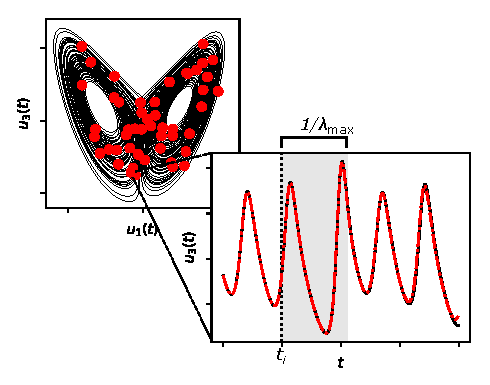
\includegraphics[width=0.6\textwidth]{figures/nrmse-avg}
  \caption{Summary of the forecasting evaluation method. I calculate
    errors $\epsilon_{1,i}$ at times $t_i$, marked on the attractor as
    red dots, and combine them into a single error
    $\tilde{\epsilon}$. Before each $t_i$ (dotted vertical line), the
    reservoir is integrated with \cref{eq:reservoir} and listening to
    the input. After $t_i$, the reservoir is integrated with
    \cref{eq:reservoir-auto}, and runs autonomously. The reservoir's
    prediction (dotted red line) must eventually diverge from the true
    system (solid black line). I calculate each $\epsilon_{1,i}$ only
    during a single Lyapunov period after forecasting begins, marked
    here in grey.}%
  \label{fig:nrmse-avg}
\end{figure}

A simple fix is to perform $k$ forecasts with many different example
inputs, calculate an $\epsilon_1$ value for each forecast, and then
combine them into one final metric
\begin{equation}
  \label{eq:nrmse-avg}
  \tilde{\epsilon} = {\left( \frac{1}{k} \sum_{i=1}^k \epsilon_{1,i} \right)}^{1/2}.
\end{equation}
This method is summarized in \cref{fig:nrmse-avg}.
Using $\tilde{\epsilon}$ averages out the chance encounters with
unstable states, and as I will show in \cref{ch:low-connectivity}, is
a more reliable indicator of a forecasting RC's performance.

% FIXME talk about return map?
For forecasting, a very useful qualitative indicator of an RCs ability
to learn the input system is to use the RC in autonomous mode to
produce a very long forecast. This forecasted signal will necessarily
diverge from the true system, but both the forecast and the true
system can then be plotted side-by-side in state space. A well-trained
RC forecast will reproduce the shape of the input system's attractor,
and these plots can reveal immediate problems with the trained RC that
metrics like NRMSE sometimes mask. Still, this comparison is
completely qualitative -- it is imprecise, and not suitable to use in
an automated setting. Future research may develop a quantitative way
to measure the similarity between the RC's reconstructed attractor and
the true attractor, which would solve the problems with the current
NRMSE metric. In the meantime, visual inspection remains a useful
sanity check on the NRMSE.

\section{Summary}

Reservoir computers are a simple tool that uses an auxiliary dynamic
reservoir to transform its input. They can be trained on example data,
and that training is done very quickly using linear regression
tools. Once trained, RCs can be used in inference tasks, or in an
autonomous mode to perform system forecasting.

The RC approach is robust to the choice of reservoir system, however
the specific requirements the reservoir must have to function are
largely unknown. When an RC fails, it is difficult to know why. Recent
work on invertable generalized synchronization is an exciting path
towards learning more.

Echo state networks are a network-based reservoir choice that is easy
to simulate in software, and replicates more traditional neural
network machine learning designs. This approach uses several
metaparameters to randomly construct the internal network. As with the
general reservoirs, there is not much concrete guidance on what values
these metaparameters should have.

In \cref{ch:low-connectivity}, I will explore some of these
metaparameters, and conclude that several guidelines for ESN
construction are not necessary. I will demonstrate several RCs with
very simple internal networks that nonetheless successfully replicate
the climate of a chaotic dynamic system.
